\documentclass[11pt,]{article}
\usepackage{lmodern}
\usepackage{amssymb,amsmath}
\usepackage{ifxetex,ifluatex}
\usepackage{fixltx2e} % provides \textsubscript
\ifnum 0\ifxetex 1\fi\ifluatex 1\fi=0 % if pdftex
  \usepackage[T1]{fontenc}
  \usepackage[utf8]{inputenc}
\else % if luatex or xelatex
  \ifxetex
    \usepackage{mathspec}
  \else
    \usepackage{fontspec}
  \fi
  \defaultfontfeatures{Ligatures=TeX,Scale=MatchLowercase}
  \newcommand{\euro}{€}
\fi
% use upquote if available, for straight quotes in verbatim environments
\IfFileExists{upquote.sty}{\usepackage{upquote}}{}
% use microtype if available
\IfFileExists{microtype.sty}{%
\usepackage{microtype}
\UseMicrotypeSet[protrusion]{basicmath} % disable protrusion for tt fonts
}{}
\usepackage[margin=1in]{geometry}
\usepackage{hyperref}
\PassOptionsToPackage{usenames,dvipsnames}{color} % color is loaded by hyperref
\hypersetup{unicode=true,
            pdftitle={Issues in developing multivariable molecular signatures for guiding clinical care decisions: supplemental simulation results},
            pdfauthor={Michael C Sachs and Lisa M McShane},
            pdfborder={0 0 0},
            breaklinks=true}
\urlstyle{same}  % don't use monospace font for urls
\usepackage{natbib}
\bibliographystyle{plainnat}
\usepackage{graphicx,grffile}
\makeatletter
\def\maxwidth{\ifdim\Gin@nat@width>\linewidth\linewidth\else\Gin@nat@width\fi}
\def\maxheight{\ifdim\Gin@nat@height>\textheight\textheight\else\Gin@nat@height\fi}
\makeatother
% Scale images if necessary, so that they will not overflow the page
% margins by default, and it is still possible to overwrite the defaults
% using explicit options in \includegraphics[width, height, ...]{}
\setkeys{Gin}{width=\maxwidth,height=\maxheight,keepaspectratio}
\setlength{\parindent}{0pt}
\setlength{\parskip}{6pt plus 2pt minus 1pt}
\setlength{\emergencystretch}{3em}  % prevent overfull lines
\providecommand{\tightlist}{%
  \setlength{\itemsep}{0pt}\setlength{\parskip}{0pt}}
\setcounter{secnumdepth}{0}

%%% Use protect on footnotes to avoid problems with footnotes in titles
\let\rmarkdownfootnote\footnote%
\def\footnote{\protect\rmarkdownfootnote}

%%% Change title format to be more compact
\usepackage{titling}

% Create subtitle command for use in maketitle
\newcommand{\subtitle}[1]{
  \posttitle{
    \begin{center}\large#1\end{center}
    }
}

\setlength{\droptitle}{-2em}
  \title{Issues in developing multivariable molecular signatures for guiding
clinical care decisions: supplemental simulation results}
  \pretitle{\vspace{\droptitle}\centering\huge}
  \posttitle{\par}
  \author{Michael C Sachs$^*$ and Lisa M McShane}
  \preauthor{\centering\large\emph}
  \postauthor{\par}
  \predate{\centering\large\emph}
  \postdate{\par}
  \date{June 30, 2016}


\usepackage{setspace}

% Redefines (sub)paragraphs to behave more like sections
\ifx\paragraph\undefined\else
\let\oldparagraph\paragraph
\renewcommand{\paragraph}[1]{\oldparagraph{#1}\mbox{}}
\fi
\ifx\subparagraph\undefined\else
\let\oldsubparagraph\subparagraph
\renewcommand{\subparagraph}[1]{\oldsubparagraph{#1}\mbox{}}
\fi


\begin{document}
\maketitle

\begin{center}
\textit{Biostatistics Branch, Biometric Research Program \\
National Cancer Institute \\
9609 Medical Center Drive, MSC 9735 \\
Bethesda, MD 20892-9735 \\
Phone: 240-276-6004 \\
Email: michael.sachs@nih.gov \\
*: Corresponding Author}

\end{center}

\clearpage

\section{Additional Simulation
Results}\label{additional-simulation-results}

In the tables and figures below, \(N\) is to the number of samples, and
\(p\) is the number of variables per sample. All results are from 1000
simulation replicates.

\clearpage

\begin{table}

\caption{Comparison of different approaches to estimating the Area Under the ROC Curve (AUC) and the log odds ratio (OR) in the setting where a dataset is used to both develop the signature and evaluate its performance. The true value of the AUC is 0.5 and the true value of the Log OR is 0.0. Estimates are based on 1000 replicates of the numerical experiment. In each replicate,  N = 1000; p = 10 . CV = Cross validation. }
\centering
\begin{tabular}[t]{l|r|r|r|r|r|r}
\hline
Approach & mean AUC & std.dev AUC & Bias AUC & mean OR & std.dev OR & Bias OR\\
\hline
Resubstitution & 0.56 & 0.01 & 0.06 & 0.34 & 0.12 & 0.34\\
\hline
Partial CV & 0.50 & 0.03 & 0.00 & -0.01 & 0.18 & -0.01\\
\hline
Partial Holdout & 0.50 & 0.03 & 0.00 & 0.00 & 0.20 & 0.00\\
\hline
Partial Resubstitution & 0.54 & 0.02 & 0.04 & 0.24 & 0.13 & 0.24\\
\hline
Pre-validation & 0.49 & 0.03 & -0.01 & -0.02 & 0.18 & -0.02\\
\hline
Leave 10 out CV & 0.50 & 0.03 & 0.00 & 0.01 & 0.18 & 0.01\\
\hline
Leave 100 out CV & 0.50 & 0.03 & 0.00 & 0.00 & 0.17 & 0.00\\
\hline
30\% Holdout & 0.50 & 0.04 & 0.00 & -0.01 & 0.24 & -0.01\\
\hline
50\% Holdout & 0.50 & 0.03 & 0.00 & 0.00 & 0.19 & 0.00\\
\hline
Bootstrap & 0.50 & 0.02 & 0.00 & 0.00 & 0.11 & 0.00\\
\hline
\end{tabular}
\end{table}

\begin{table}

\caption{Comparison of different approaches to estimating the Area Under the ROC Curve (AUC) and the log odds ratio (OR) in the setting where a dataset is used to both develop the signature and evaluate its performance. The true value of the AUC is 0.5 and the true value of the Log OR is 0.0. Estimates are based on 1000 replicates of the numerical experiment. In each replicate,  N = 1000; p = 100 . CV = Cross validation. }
\centering
\begin{tabular}[t]{l|r|r|r|r|r|r}
\hline
Approach & mean AUC & std.dev AUC & Bias AUC & mean OR & std.dev OR & Bias OR\\
\hline
Resubstitution & 0.66 & 0.01 & 0.16 & 0.95 & 0.12 & 0.95\\
\hline
Partial CV & 0.61 & 0.02 & 0.11 & 0.59 & 0.13 & 0.59\\
\hline
Partial Holdout & 0.59 & 0.03 & 0.09 & 0.51 & 0.19 & 0.51\\
\hline
Partial Resubstitution & 0.61 & 0.02 & 0.11 & 0.66 & 0.13 & 0.66\\
\hline
Pre-validation & 0.50 & 0.04 & 0.00 & -0.02 & 0.26 & -0.02\\
\hline
Leave 10 out CV & 0.50 & 0.04 & 0.00 & 0.00 & 0.21 & 0.00\\
\hline
Leave 100 out CV & 0.50 & 0.03 & 0.00 & 0.00 & 0.19 & 0.00\\
\hline
30\% Holdout & 0.50 & 0.03 & 0.00 & 0.00 & 0.25 & 0.00\\
\hline
50\% Holdout & 0.50 & 0.03 & 0.00 & 0.00 & 0.20 & 0.00\\
\hline
Bootstrap & 0.50 & 0.02 & 0.00 & 0.00 & 0.10 & 0.00\\
\hline
\end{tabular}
\end{table}

\begin{table}

\caption{Comparison of different approaches to estimating the Area Under the ROC Curve (AUC) and the log odds ratio (OR) in the setting where a dataset is used to both develop the signature and evaluate its performance. The true value of the AUC is 0.5 and the true value of the Log OR is 0.0. Estimates are based on 1000 replicates of the numerical experiment. In each replicate,  N = 1000; p = 500 . CV = Cross validation. }
\centering
\begin{tabular}[t]{l|r|r|r|r|r|r}
\hline
Approach & mean AUC & std.dev AUC & Bias AUC & mean OR & std.dev OR & Bias OR\\
\hline
Resubstitution & 0.72 & 0.01 & 0.22 & 1.33 & 0.11 & 1.33\\
\hline
Partial CV & 0.68 & 0.01 & 0.18 & 1.03 & 0.11 & 1.03\\
\hline
Partial Holdout & 0.66 & 0.02 & 0.16 & 0.96 & 0.18 & 0.96\\
\hline
Partial Resubstitution & 0.65 & 0.02 & 0.15 & 0.89 & 0.13 & 0.89\\
\hline
Pre-validation & 0.50 & 0.06 & 0.00 & -0.01 & 0.33 & -0.01\\
\hline
Leave 10 out CV & 0.50 & 0.04 & 0.00 & 0.00 & 0.25 & 0.00\\
\hline
Leave 100 out CV & 0.50 & 0.03 & 0.00 & 0.00 & 0.21 & 0.00\\
\hline
30\% Holdout & 0.50 & 0.03 & 0.00 & 0.00 & 0.24 & 0.00\\
\hline
50\% Holdout & 0.50 & 0.03 & 0.00 & 0.00 & 0.20 & 0.00\\
\hline
Bootstrap & 0.50 & 0.01 & 0.00 & 0.00 & 0.08 & 0.00\\
\hline
\end{tabular}
\end{table}

\begin{table}

\caption{Comparison of different approaches to estimating the Area Under the ROC Curve (AUC) and the log odds ratio (OR) in the setting where a dataset is used to both develop the signature and evaluate its performance. The true value of the AUC is 0.5 and the true value of the Log OR is 0.0. Estimates are based on 1000 replicates of the numerical experiment. In each replicate,  N = 200; p = 10 . CV = Cross validation. }
\centering
\begin{tabular}[t]{l|r|r|r|r|r|r}
\hline
Approach & mean AUC & std.dev AUC & Bias AUC & mean OR & std.dev OR & Bias OR\\
\hline
Resubstitution & 0.63 & 0.03 & 0.13 & 0.78 & 0.27 & 0.78\\
\hline
Partial CV & 0.50 & 0.08 & 0.00 & -0.01 & 0.35 & -0.01\\
\hline
Partial Holdout & 0.50 & 0.06 & 0.00 & -0.02 & 0.43 & -0.02\\
\hline
Partial Resubstitution & 0.60 & 0.04 & 0.10 & 0.56 & 0.31 & 0.56\\
\hline
Pre-validation & 0.50 & 0.06 & 0.00 & 0.02 & 0.40 & 0.02\\
\hline
Leave 10 out CV & 0.50 & 0.08 & 0.00 & 0.00 & 0.34 & 0.00\\
\hline
Leave 100 out CV & 0.50 & 0.07 & 0.00 & 0.00 & 0.39 & 0.00\\
\hline
30\% Holdout & 0.50 & 0.08 & 0.00 & 0.02 & 0.53 & 0.02\\
\hline
50\% Holdout & 0.50 & 0.06 & 0.00 & 0.01 & 0.43 & 0.01\\
\hline
Bootstrap & 0.50 & 0.04 & 0.00 & -0.01 & 0.24 & -0.01\\
\hline
\end{tabular}
\end{table}

\begin{table}

\caption{Comparison of different approaches to estimating the Area Under the ROC Curve (AUC) and the log odds ratio (OR) in the setting where a dataset is used to both develop the signature and evaluate its performance. The true value of the AUC is 0.5 and the true value of the Log OR is 0.0. Estimates are based on 1000 replicates of the numerical experiment. In each replicate,  N = 200; p = 100 . CV = Cross validation. }
\centering
\begin{tabular}[t]{l|r|r|r|r|r|r}
\hline
Approach & mean AUC & std.dev AUC & Bias AUC & mean OR & std.dev OR & Bias OR\\
\hline
Resubstitution & 0.84 & 0.03 & 0.34 & 2.32 & 0.37 & 2.32\\
\hline
Partial CV & 0.71 & 0.04 & 0.21 & 1.21 & 0.34 & 1.21\\
\hline
Partial Holdout & 0.67 & 0.06 & 0.17 & 1.00 & 0.45 & 1.00\\
\hline
Partial Resubstitution & 0.72 & 0.04 & 0.22 & 1.40 & 0.33 & 1.40\\
\hline
Pre-validation & 0.50 & 0.07 & 0.00 & 0.01 & 0.41 & 0.01\\
\hline
Leave 10 out CV & 0.50 & 0.07 & 0.00 & 0.00 & 0.41 & 0.00\\
\hline
Leave 100 out CV & 0.50 & 0.07 & 0.00 & 0.03 & 0.43 & 0.03\\
\hline
30\% Holdout & 0.49 & 0.08 & -0.01 & -0.04 & 0.52 & -0.04\\
\hline
50\% Holdout & 0.50 & 0.06 & 0.00 & 0.00 & 0.44 & 0.00\\
\hline
Bootstrap & 0.50 & 0.04 & 0.00 & -0.01 & 0.21 & -0.01\\
\hline
\end{tabular}
\end{table}

\begin{table}

\caption{Comparison of different approaches to estimating the Area Under the ROC Curve (AUC) and the log odds ratio (OR) in the setting where a dataset is used to both develop the signature and evaluate its performance. The true value of the AUC is 0.5 and the true value of the Log OR is 0.0. Estimates are based on 1000 replicates of the numerical experiment. In each replicate,  N = 200; p = 500 . CV = Cross validation. }
\centering
\begin{tabular}[t]{l|r|r|r|r|r|r}
\hline
Approach & mean AUC & std.dev AUC & Bias AUC & mean OR & std.dev OR & Bias OR\\
\hline
Resubstitution & 0.92 & 0.02 & 0.42 & 3.42 & 0.58 & 3.42\\
\hline
Partial CV & 0.83 & 0.03 & 0.33 & 2.07 & 0.30 & 2.07\\
\hline
Partial Holdout & 0.76 & 0.07 & 0.26 & 1.77 & 0.54 & 1.77\\
\hline
Partial Resubstitution & 0.74 & 0.03 & 0.24 & 1.62 & 0.30 & 1.62\\
\hline
Pre-validation & 0.50 & 0.08 & 0.00 & 0.00 & 0.48 & 0.00\\
\hline
Leave 10 out CV & 0.50 & 0.07 & 0.00 & 0.02 & 0.45 & 0.02\\
\hline
Leave 100 out CV & 0.50 & 0.08 & 0.00 & 0.00 & 0.45 & 0.00\\
\hline
30\% Holdout & 0.50 & 0.08 & 0.00 & 0.00 & 0.54 & 0.00\\
\hline
50\% Holdout & 0.50 & 0.05 & 0.00 & 0.03 & 0.45 & 0.03\\
\hline
Bootstrap & 0.50 & 0.03 & 0.00 & 0.00 & 0.17 & 0.00\\
\hline
\end{tabular}
\end{table}

\begin{table}

\caption{Comparison of different approaches to estimating the Area Under the ROC Curve (AUC) and the log odds ratio (OR) in the setting where a dataset is used to both develop the signature and evaluate its performance. The true value of the AUC is 0.5 and the true value of the Log OR is 0.0. Estimates are based on 1000 replicates of the numerical experiment. In each replicate,  N = 200; p = 5000 . CV = Cross validation. }
\centering
\begin{tabular}[t]{l|r|r|r|r|r|r}
\hline
Approach & mean AUC & std.dev AUC & Bias AUC & mean OR & std.dev OR & Bias OR\\
\hline
Resubstitution & 0.97 & 0.01 & 0.47 & 4.86 & 0.77 & 4.86\\
\hline
Partial CV & 0.90 & 0.02 & 0.40 & 2.75 & 0.27 & 2.75\\
\hline
Partial Holdout & 0.80 & 0.06 & 0.30 & 2.53 & 0.68 & 2.53\\
\hline
Partial Resubstitution & 0.76 & 0.03 & 0.26 & 1.62 & 0.33 & 1.62\\
\hline
Pre-validation & 0.50 & 0.06 & 0.00 & 0.00 & 0.43 & 0.00\\
\hline
Leave 10 out CV & 0.50 & 0.07 & 0.00 & 0.00 & 0.44 & 0.00\\
\hline
Leave 100 out CV & 0.49 & 0.09 & -0.01 & -0.05 & 0.51 & -0.05\\
\hline
30\% Holdout & 0.50 & 0.06 & 0.00 & 0.03 & 0.55 & 0.03\\
\hline
50\% Holdout & 0.51 & 0.06 & 0.01 & 0.06 & 0.43 & 0.06\\
\hline
Bootstrap & 0.50 & 0.02 & 0.00 & -0.01 & 0.13 & -0.01\\
\hline
\end{tabular}
\end{table}

\clearpage

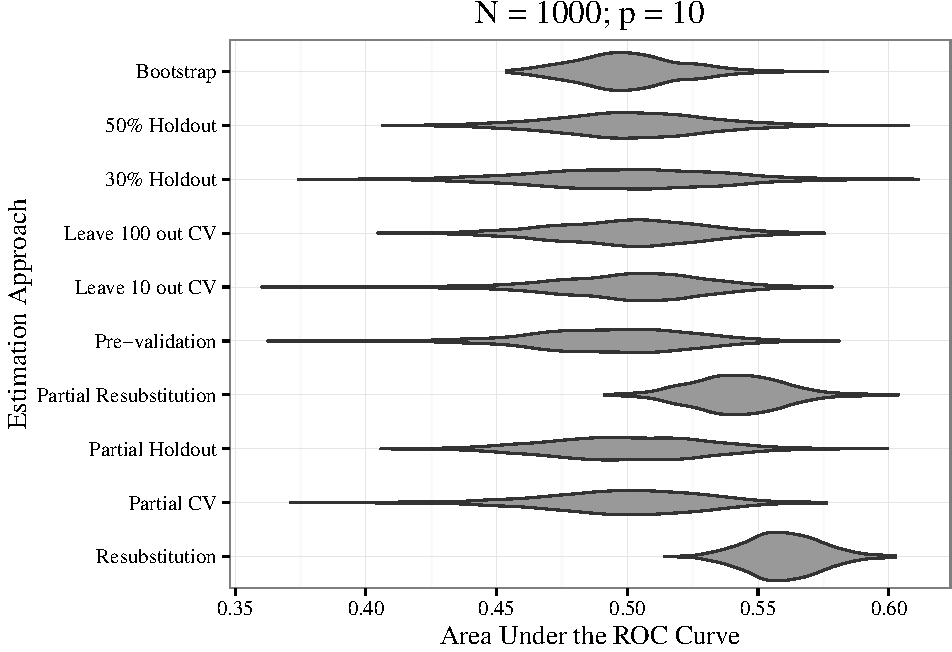
\includegraphics{supplement_files/figure-latex/plotsauc-1.pdf}
\clearpage

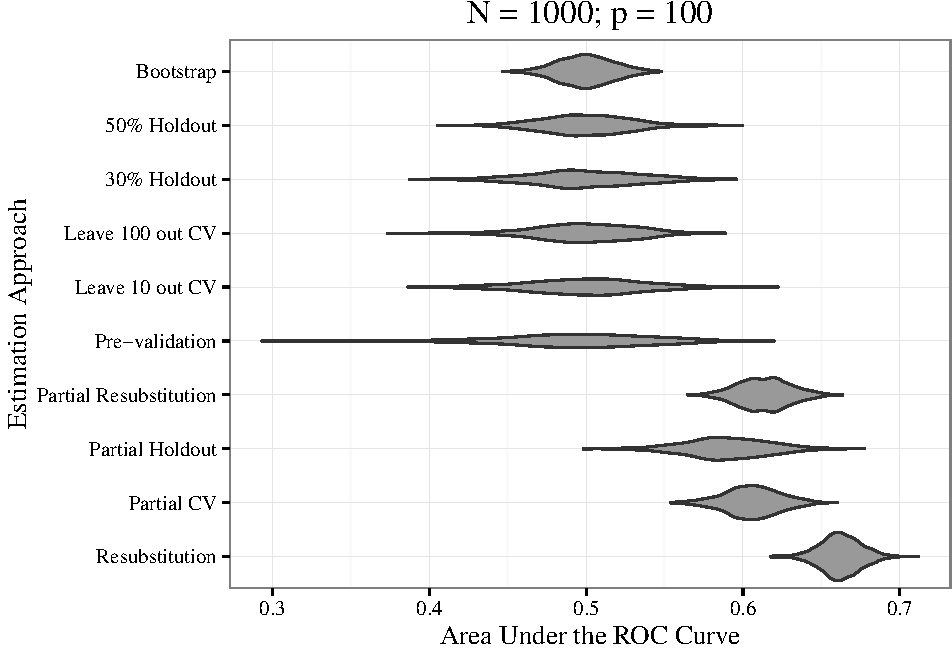
\includegraphics{supplement_files/figure-latex/plotsauc-2.pdf}
\clearpage

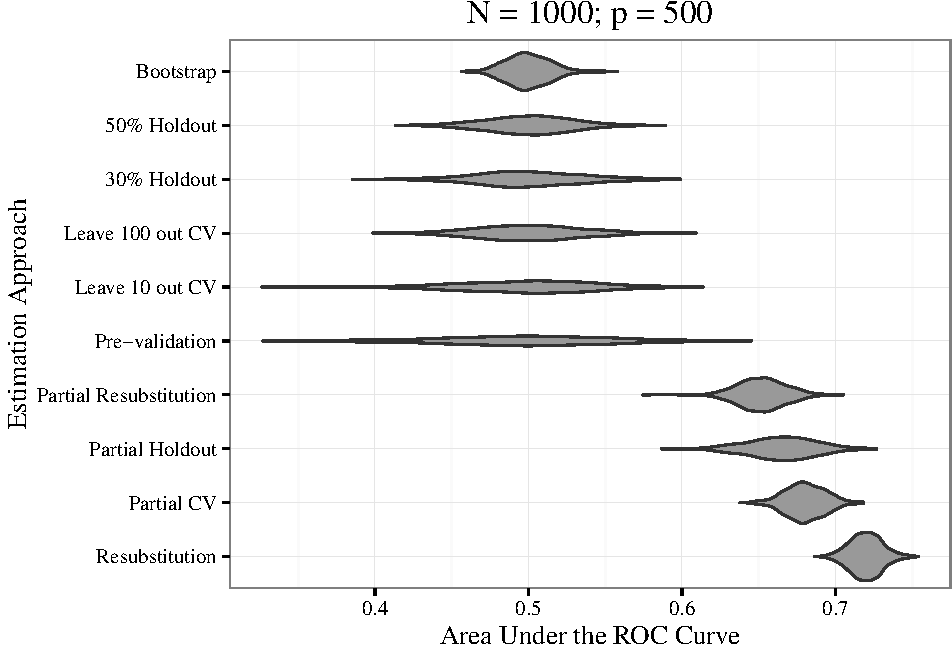
\includegraphics{supplement_files/figure-latex/plotsauc-3.pdf}
\clearpage

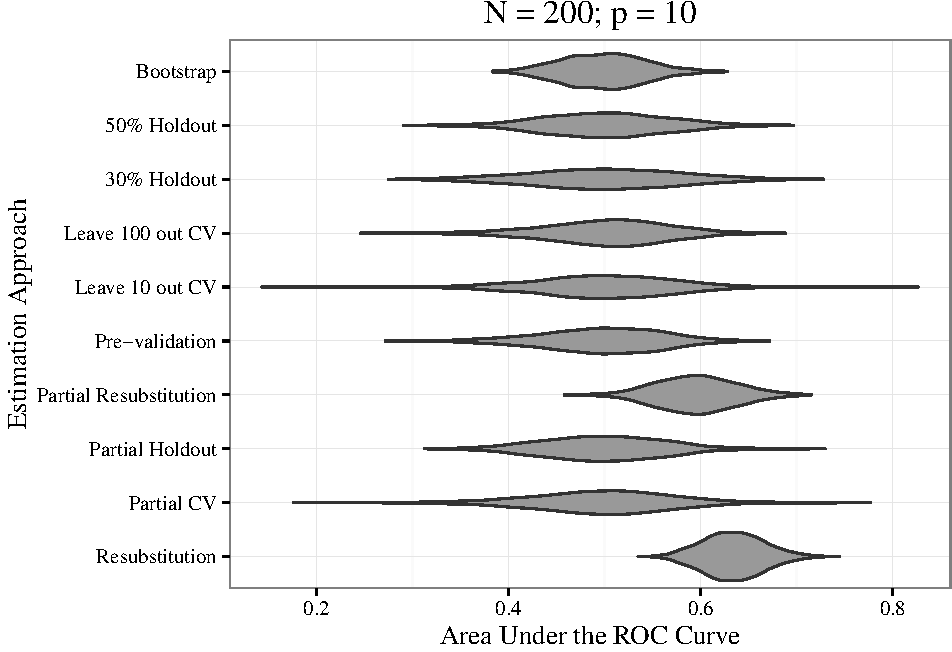
\includegraphics{supplement_files/figure-latex/plotsauc-4.pdf}
\clearpage

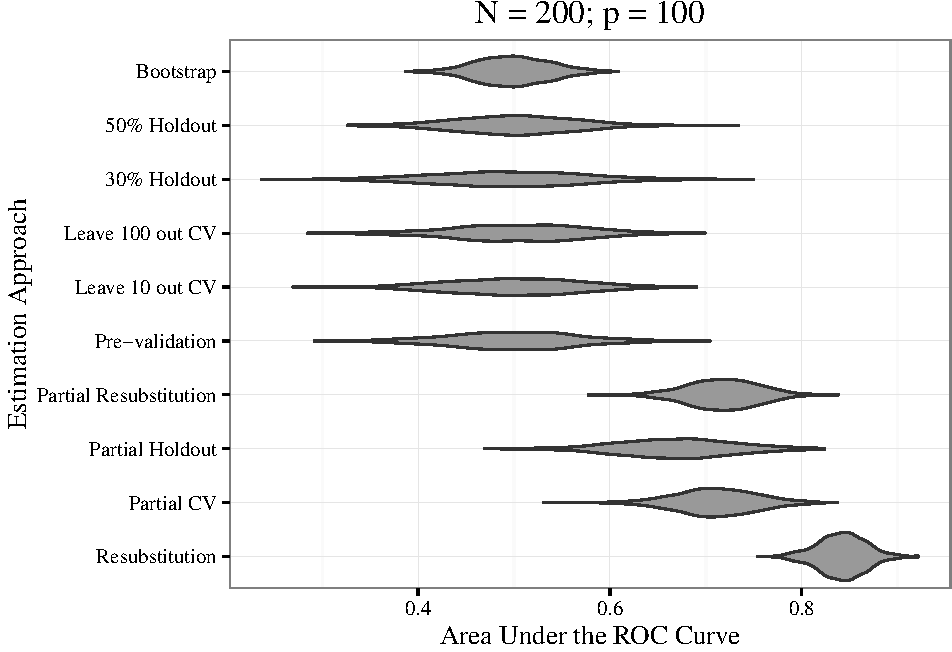
\includegraphics{supplement_files/figure-latex/plotsauc-5.pdf}
\clearpage

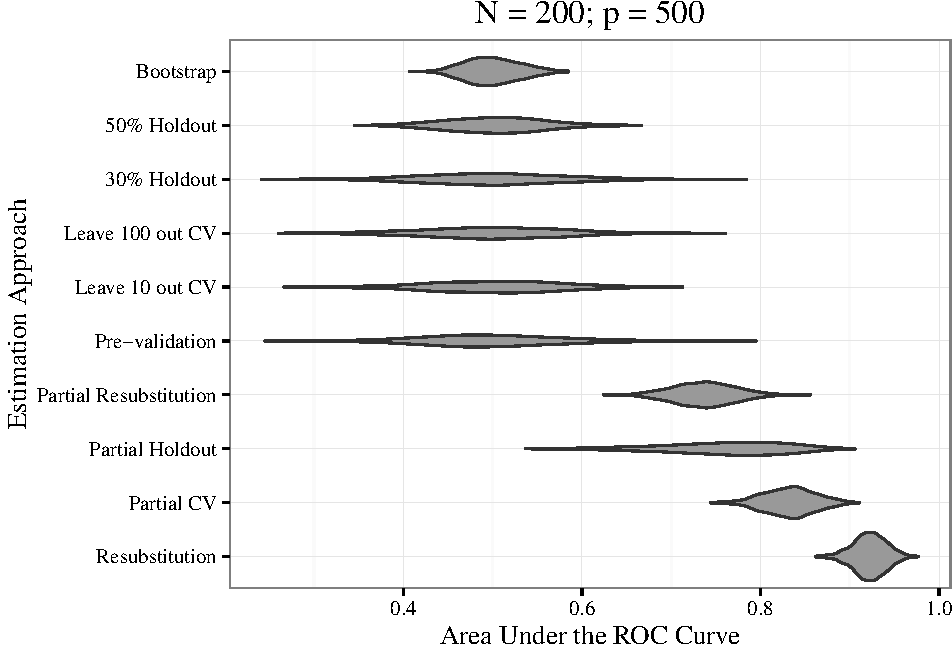
\includegraphics{supplement_files/figure-latex/plotsauc-6.pdf}
\clearpage

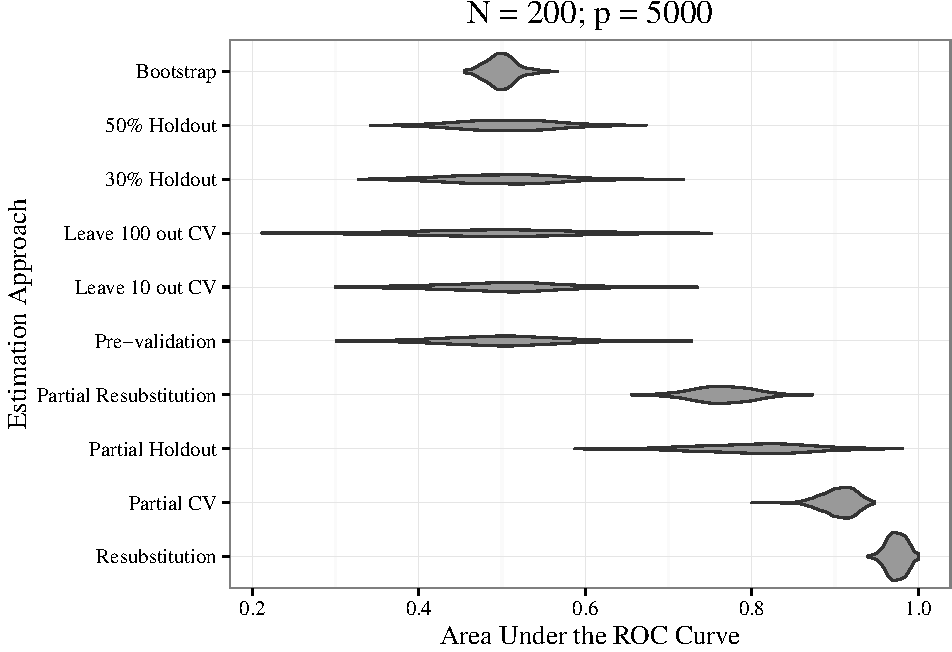
\includegraphics{supplement_files/figure-latex/plotsauc-7.pdf}
\clearpage

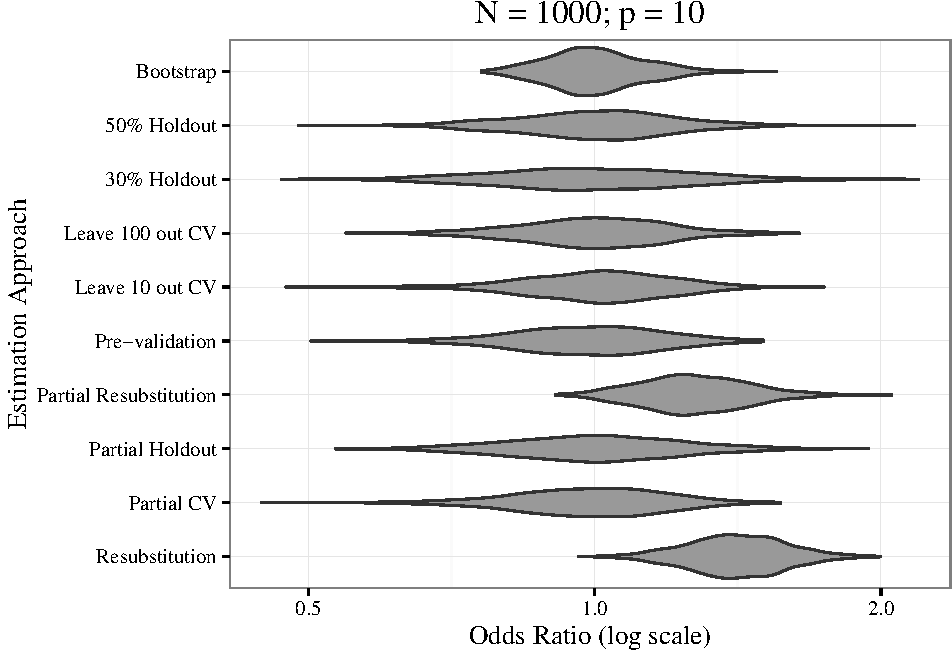
\includegraphics{supplement_files/figure-latex/plots2-1.pdf} \clearpage

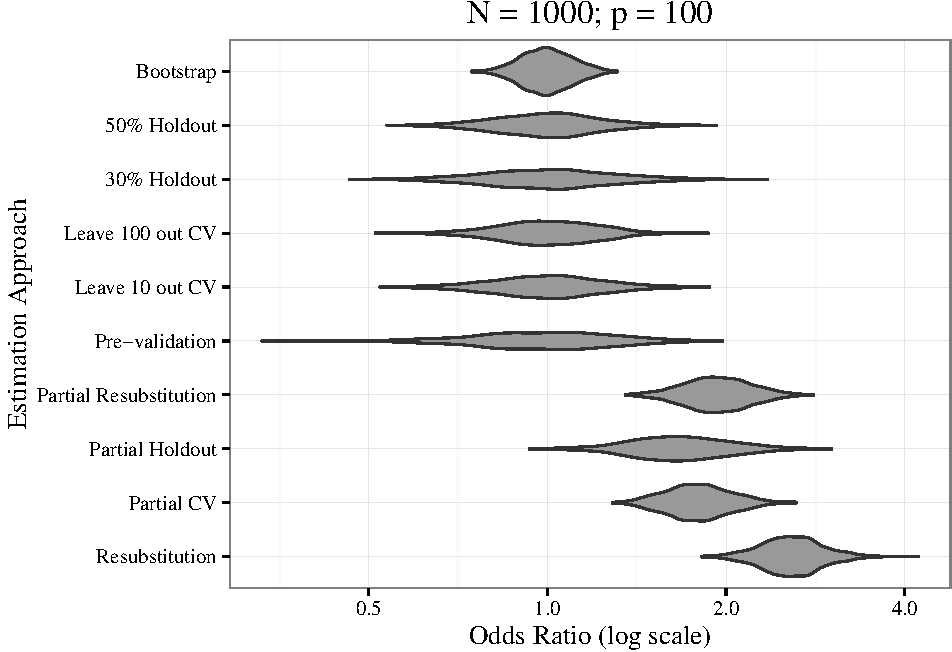
\includegraphics{supplement_files/figure-latex/plots2-2.pdf} \clearpage

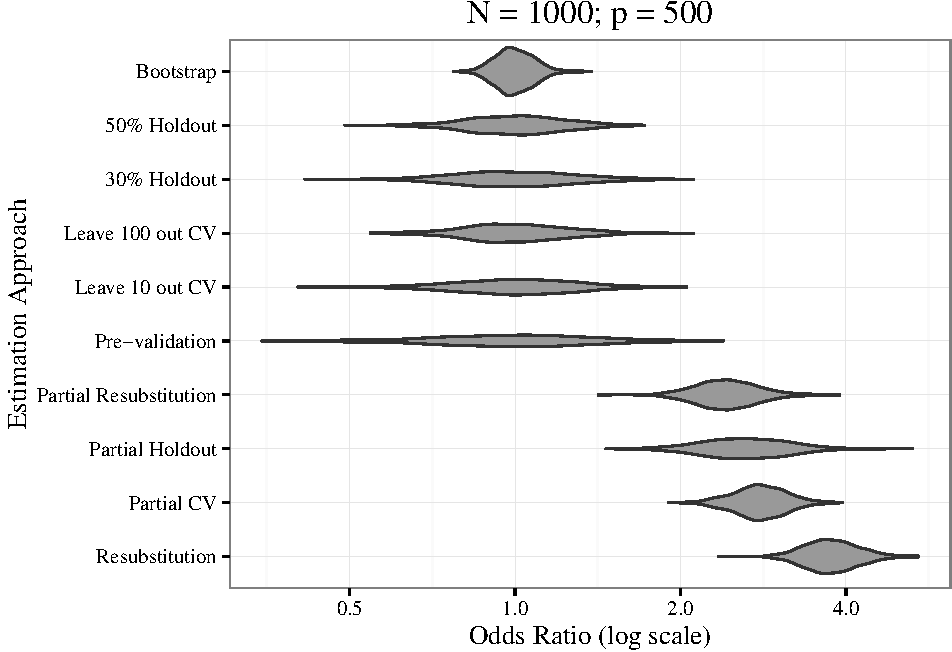
\includegraphics{supplement_files/figure-latex/plots2-3.pdf} \clearpage

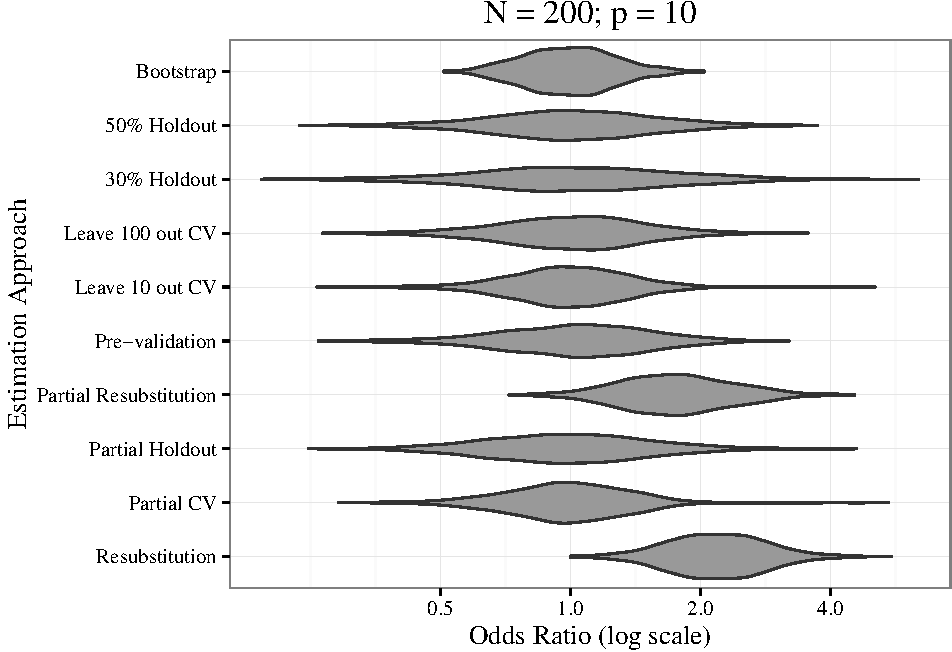
\includegraphics{supplement_files/figure-latex/plots2-4.pdf} \clearpage

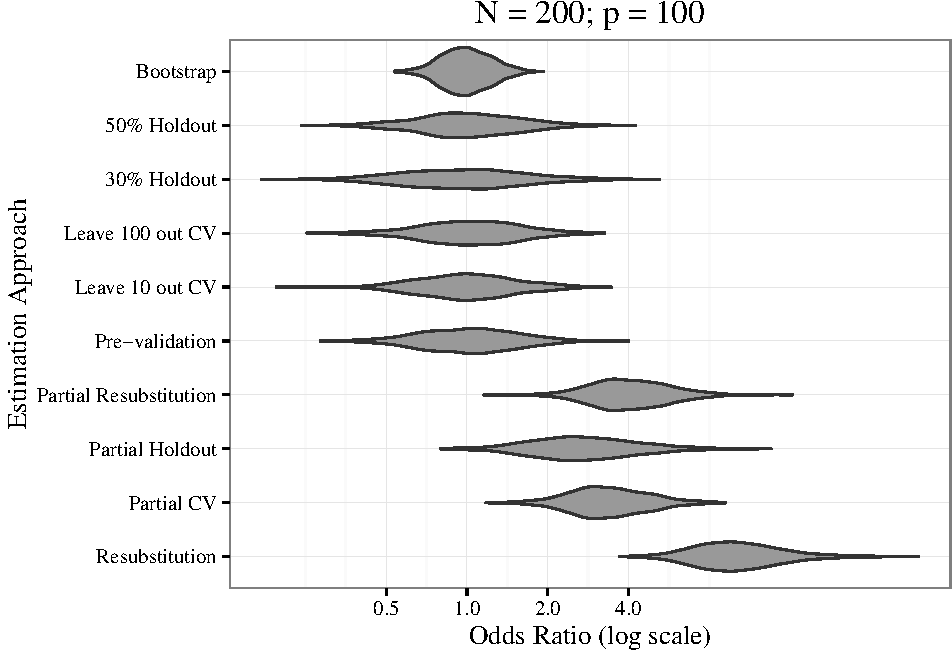
\includegraphics{supplement_files/figure-latex/plots2-5.pdf} \clearpage

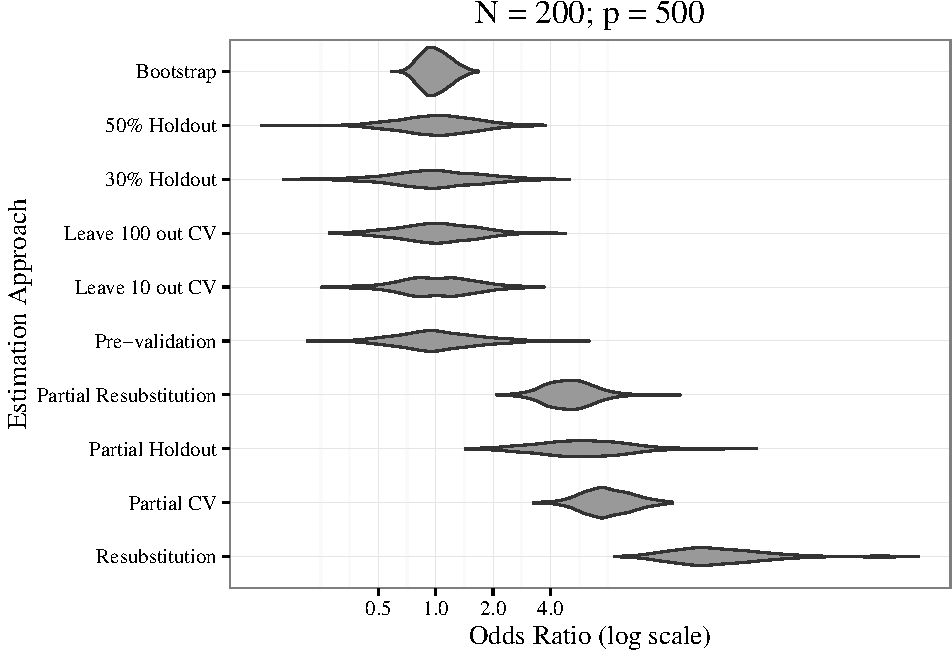
\includegraphics{supplement_files/figure-latex/plots2-6.pdf} \clearpage

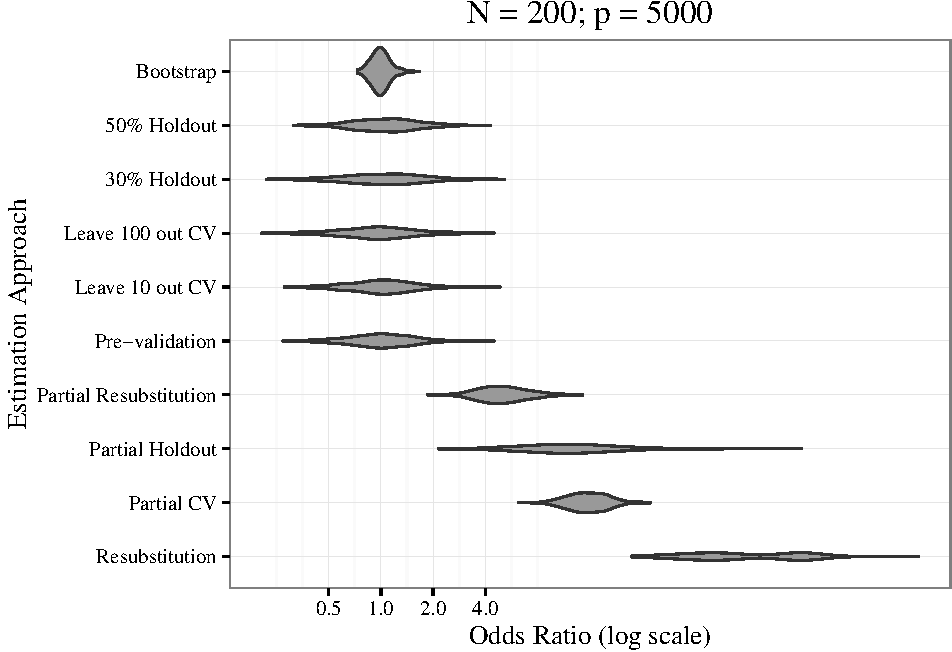
\includegraphics{supplement_files/figure-latex/plots2-7.pdf} \clearpage

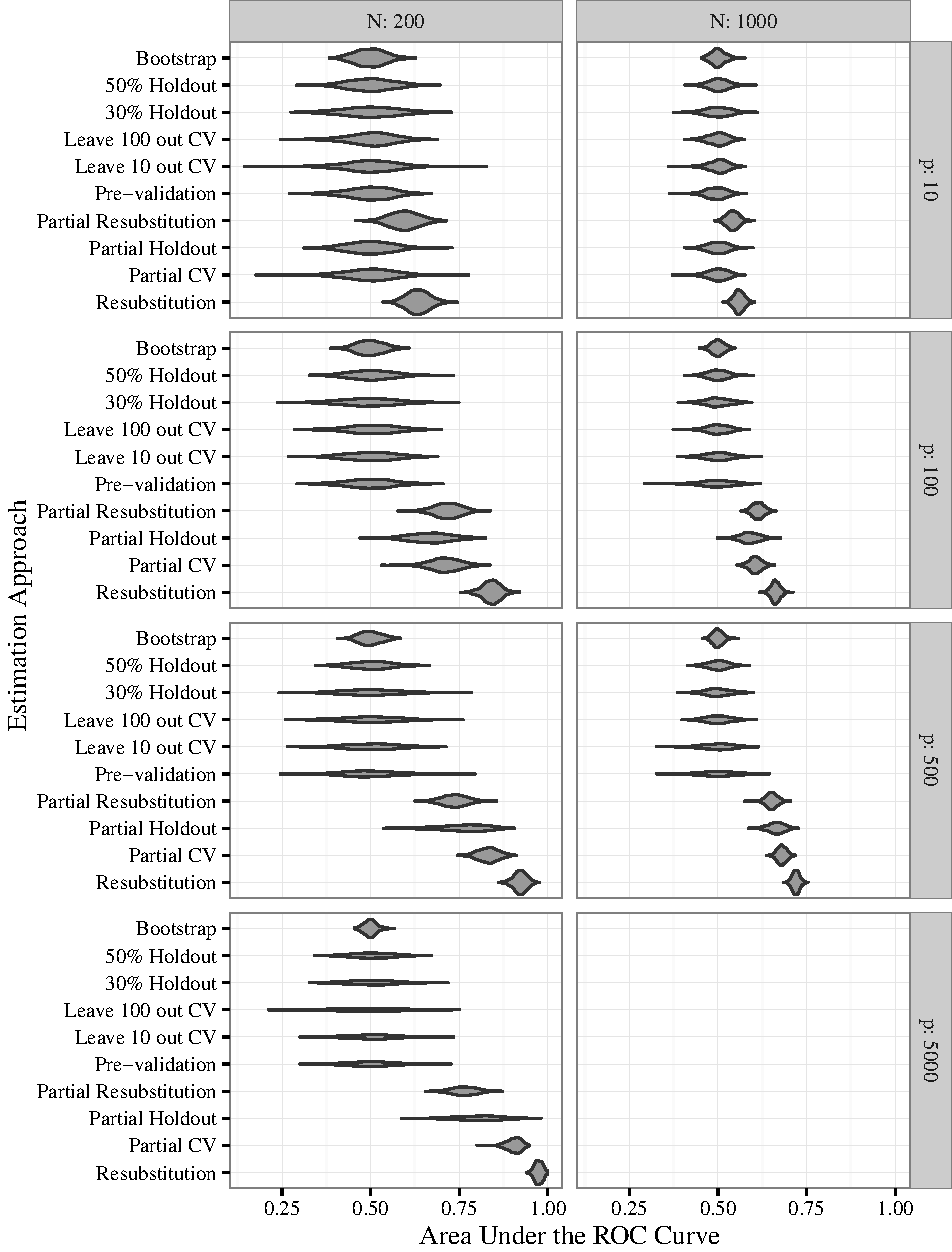
\includegraphics{supplement_files/figure-latex/overall-1.pdf}

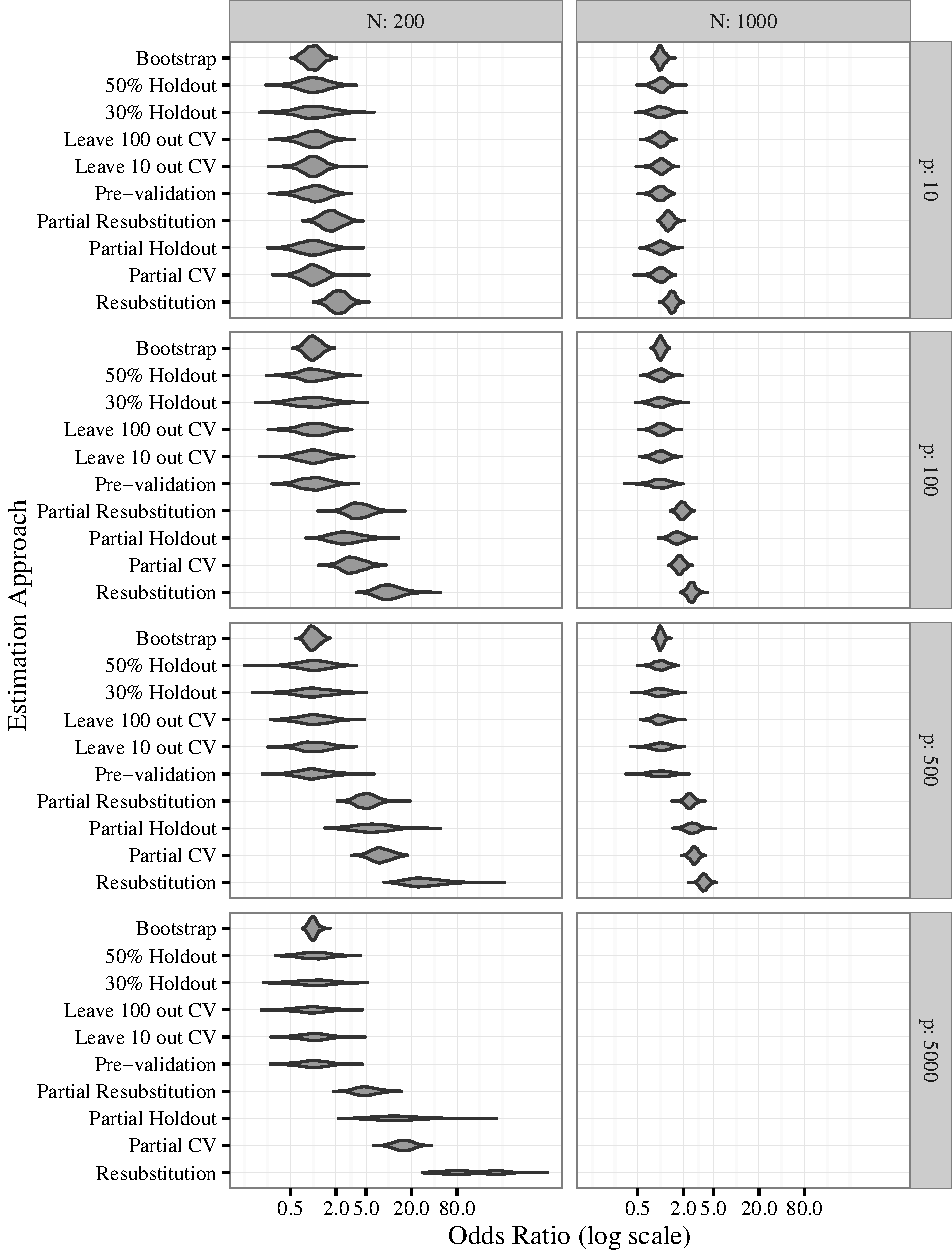
\includegraphics{supplement_files/figure-latex/unnamed-chunk-1-1.pdf}

\bibliography{paper.bib}

\end{document}
